%%=============================================================================
%% Inleiding
%%=============================================================================

\chapter{Inleiding}
\label{ch:inleiding}

\section{Stand van zaken}
\label{sec:stand-van-zaken}

\begin{itemize}
	\item Gebruiken in de taal die je wilt (ondersteunde talen zijn: Curl, Java, C\#, Python, JavaScript, PHP, Perl, Ruby)
	
	Wie gebruikt het? 
	
	Enkele merkwaardige gebruikers van Elasticsearch zijn NASA, Netflix, Github, Facebook, Cisco, Microsoft en Adobe. Ook Zalando, Just Eat, Blizzard, Ebay, Warner Brothers, BBC, Walmart, Uber, Tinder, Mozilla, Activision, Orange, ... (bron https://www.elastic.co/use-cases)
	
\end{itemize}

Elasticsearch is een zoekmachine die in Java geschreven is. De zoekmachine werd boven de Java library Apache Lucene gebouwd. Alle commando's worden verzonden door middel van HTTP requests naar de Elasticsearch REST API. Die API is gebaseerd op JSON. Dat wil zeggen dat de mogelijkheid bestaat om JSON mee te geven aan de HTTP requests. Ook de resultaten worden in JSON teruggegeven. Elasticsearch is niet enkel een zoekmachine maar wordt ook gebruikt voor data-analyses en om aan logging te doen. 

Shay Bannon ontwierp Elasticsearch als een gedistribueerd systeem. Een gedistribueerd systeem brengt zowel voordelen als nadelen met zich mee. Volgens \textcite{Brasetvik2013} focussen verschillende systemen op verschillende sterktes, afhankelijk van welke eigenschappen belangrijker zijn voor het systeem. Daarbij wordt gezegd dat Elasticsearch focust op snelheid. Het streeft naar real-time search. Om dat de kunnen bereiken in een gedistribueerd systeem worden een aantal zaken aan de kant geschoven of vereenvoudigd. Een voorbeeld hiervan is concurrency control. Die wordt gedaan aan de hand van versienummers van de documents. Dit is wat we noemen een optimistische aanpak. Deze heeft als voordeel dat het sneller gaat maar in uitzonderlijke gevallen kan dit foute resultaten in de zoekopdrachten en data-analyses opleveren. In een zoekopdracht is het misschien nog aanvaardbaar dat sommige resultaten niet worden weergegeven. Zeker als dat ervoor zorgt dat men over real-time search kan spreken. In een data-analyse is het echter zeer belangrijk dat de resultaten correct zijn. Een tweede manier om aan snelheid te winnen in een gedistribueerd systeem is caching. Elasticsearch doet vaak aan caching om niet telkens opnieuw alle data te moeten opvragen. Dat heeft een negatief effect op het geheugen dat het systeem nodig heeft maar ook een zeer positief effect op de uitvoeringstijd.

Het CAP theorema stelt dat het onmogelijk is voor een gedistribueerd systeem om gelijktijdig consistent (C), beschikbaar (A) en partitie tolerant (P) te zijn. Het stelt dat een gedistribueerd systeem aan maximaal twee van de voorgenoemde eigenschappen kan voldoen. Consistent betekent dat alle nodes in de cluster dezelfde data zien op hetzelfde moment. Daarbij is het belangrijk dat deze data de meest recente data is. Men kan spreken over een beschikbaar systeem wanneer alle nodes een reponse kunnen geven voor alle requests. Wanneer een node geen response kan geven op een request wordt er niet aan de criteria voldaan om over een beschikbaar systeem te kunnen spreken. De laatste voorwaarde in het CAP theorema, partitie tolerant, houdt in dat het systeem correct blijft functioneren bij het uitvallen van een node in het netwerk. Volgens \textcite{Brasetvik2013} is het bij Elasticsearch over het algemeen zo dat het systeem consistent en partitie tolerant is. Dat noemt men een CP-systeem. Hierbij is het niet onbelangrijk om te vermelden dat er een zwakke definitie voor consistentie gebruikt wordt. Wat er precies gegarandeerd wordt is document consistentie waarbij er sprake is van consistentie binnen een document. Wanneer men Elasticsearch enkel gebruikt om data uit te lezen bereikt men een systeem dat beschikbaar en partitie tolerant is. Dat noemt men een AP-systeem.

\textcite{Glauner2012} schrijft dat één van de belangrijkste sterktes van de zoekmachine is dat het gebruik maakt van een schema-less data model. Hierdoor kan elk JSON document aan Elasticsearch toegevoegd worden. Dat zorgt voor veel flexibiliteit en minder configuratiewerk voor de gebruikers. \textcite{Brasetvik2013} gebruikt liever de term schema flexible. Er is namelijk wel een schema, alleen moet die niet verplicht meegegeven worden. De zoekmachine is zeer sterk in het herkennen van eenvoudige datatypes zoals nummers, booleans en timestamps. Daardoor kan het schema gegenereerd worden zonder expliciet te moeten meegeven wat de datatypes zijn. De mogelijkheid om een schema mee te geven bestaat echter wel. Een reden om zelf een schema mee te geven is om de data op punt te stellen en zo de zoeksnelheden te doen laten stijgen.

\subsection{Elasticsearch archeologie}

Om dit onderzoek beter te begrijpen worden de belangrijkste termen uit de archeologie van Elasticsearch bekeken. In het boek \textcite{Dixit2016} leert men hoe de archeologie van Elasticsearch in elkaar zit. Daarin staat dat een cluster een verzameling van nodes is die met elkaar verbonden zijn. De eerste cluster heeft standaard Elasticsearch als naam. Alle clusters samen stellen uw data voor. In figuur \ref{fig:ESArchitecture} van \textcite{Babaev2013} is te zien hoe zo'n cluster in elkaar zit. Een node is een instantie van Elasticsearch. Bij de creatie krijgt een node standaard een UUID en komt bij de Elasticsearch cluster tenzij anders gedefinieerd. In de zitten de indices. Een index is een verzameling van documents met gelijkaardige karakteristieken. Hier slaat Elasticsearch data in op. Een index kan zeer groot worden. Het kan gebeuren dat de index te groot wordt om op de schijf van een node op te slaan. Daarom bestaat een index uit meerdere shards en replicas. Deze worden door Elasticsearch voorzien om een index op te delen in stukken. Een shard kan een primaire shard of een secundaire shard zijn. Operaties die data aanpassen gebeuren op primaire shards. Secundaire shards bevatten kopies van de data van de primaire shards en zorgt ervoor dat het zoeken snel gebeurd. Kopies van data bewaren heeft ook als effect dat er sprake is van een hoge beschikbaarheid. Wanneer een primaire shard stopgezet wordt sprint een secundaire shard in om de rol van de primaire shard te vervangen. Een veelgebruikt synoniem voor een secundaire shard is replica. Als laatste zijn er documents. Een document is een JSON object dat de key-value paren bevat van één object.

\begin{figure}
	\centering
	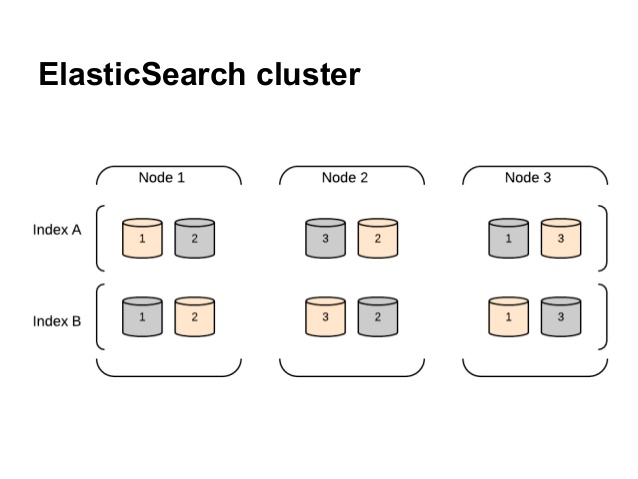
\includegraphics[width= 10cm]{ESArchitecture}
	\caption{Een cluster in Elasticsearch}
	\label{fig:ESArchitecture}
\end{figure}

\subsection{Schaalbaarheid}

In de master thesis van \textcite{Berglund2013} wordt er een belangrijke stelling gemaakt over de schaalbaarheid van Elasticsearch. De search engine is zeer schaalbaar omdat de documents organisatorisch verdeeld zijn over verschillende nodes. Bij een specifieke zoekopdracht waarbij men zoekt op het document ID of het type zullen slechts enkele nodes moeten overlopen worden. Dat ideale scenario is echter niet altijd relevant. Afhankelijk van de criteria waarop men zoekt, kan het zijn dat alle nodes moeten overlopen worden. Dat is een limitatie van de schaalbaarheid van Elasticsearch. Dat probleem zou vandaag nog niet opgelost kunnen worden zonder dat er data-verlies voorkomt in de zoekresultaten. Zeer sterk in schaalbaarheid. Bij het toevoegen van een nieuwe node worden de shards verplaatst zodat de nodige opslagruimte minimaal blijft.  

Distributed: Elasticsearch is distributed in nature from day one, and has been designed for scaling horizontally and not vertically. You can start with a single-node Elasticsearch cluster on your laptop and can scale that cluster to hundreds or thousands of nodes without worrying about the internal complexities that come with distributed computing, distributed document storage, and searches. DIXIT

\subsection{Installatie}
\label{Installatie}

Elasticsearch is gratis als je beslist om het zelf te hosten. De installatie verloopt zeer snel. Eerst moet je zorgen dat Java geïnstalleerd staat op je computer. Daarna download je een versie van Elasticsearch naar keuze via de website. Pak het bestand uit en je bent klaar om je eerste cluster op te zetten. Als dat te moeilijk is kan men gebruik maken van een grafische user interface die beschikbaar is via de MSI installer package. Op de website staat stap voor stap uitgelegd hoe je de installatie kunt uitvoeren. 


Er hangen niet zoveel nadelen vast aan het zelf hosten van Elasticsearch. Je moet natuurlijk wel over voldoende ruimte beschikken op je harde schijf. Dat kan moeilijk worden wanneer men met grote hoeveelheden data werkt. Daarnaast is het belangrijk om te weten dat je zelf verantwoordelijk bent voor eventuele downtimes. Het is dus perfect mogelijk om Elasticsearch volledig gratis te gebruiken. 

Wanneer men beslist om te betalen voor de hosting bij Elasticsearch beschikt men wel over enkele voordelen . De eerder vermelde problemen in verband met ruimte op je harde schijf en downtimes zijn niet langer van toepassing.  Aan de hosting zijn een aantal Service Level Agreements verbonden die ervoor zorgen dat je verzekerd bent van een goede kwaliteit en dat je kan rekenen op voldoende support. De kostprijs is 36,53 EUR per maand. Er is ook een mogelijkheid om eerst een proefversie van 14 dagen te gebruiken.

\subsection{Data importeren in Elasticsearch}

Om data te exporteren van de databank naar Elasticsearch zijn er een aantal mogelijkheden, afhankelijk van welke databank er gebruik wordtt. De eerste mogelijkheid is er één die Elasticsearch zelf aanbiedt. Daarvoor maken ze gebruik van een ander product uit de Elastic Stack\footnote{De Elastic Stack is een verzameling van open-source producten van Elastic.}: Logstash. Logstash is een ETL-tool om data te verwerken, te transformeren en uit te wisselen. Het is een product waar veel informatie en support over te vinden is. Logstash is dus een tool die veel flexibiliteit biedt maar vraagt wel een extra installatie vergt. 

Daarnaast zijn er een aantal tools die aangeboden worden door de community. Voor die tools is er in het algemeen minder support te vinden. Nog een nadeel is dat het niet altijd mogelijk is om de data naar de laatste versie van Elasticsearch te exporteren. De versies van de tools lopen namelijk in het algemeen achter op de nieuwste versie van Elasticsearch. 

Zowel Logstash als de meeste tools die worden aangeboden door de community bieden ook de functionaliteit aan om data te synchroniseren. Dat wil zeggen dat, wanneer de data veranderd in de databank, die veranderingen ook doorgevoerd worden in Elasticsearch. In veel use cases zal dit veel voordelen bieden. 

\textbf{VERDERE LITERATUURSTUDIE}

\begin{itemize}
	\item Elasticsearch biedt veel features zoals full text-search, suggesties (did you mean), results highlighting, custom document scoring (relevantie berekenen bijvoorbeeld aantal matches, lengte van het veld, ...) 
	\item Open Source
	\item De query DSL van Elasticsearch is minder gebruikelijk en minder flexibel dan die van SQL. Dat betekent dat je, ondanks de hoge leercurve, minder flexibiliteit hebt.  
	\item Geen vorm van security. (alle gebruikers zijn super admin) 
	\item relaties: Bresetvik Elasticsearch is a document oriented database. The entire object graph you want to search needs to be indexed, so before indexing your documents, they must be denormalized. Denormalization increases retrieval performance (since no query joining is necessary), uses more space (because things must be stored several times), but makes keeping things consistent and up-to-date more difficult (as any change must be applied to all instances). They're excellent for write-once-read-many-workloads, however.
	\item nieuw zegt dat het poorly documented is (2012) nu wel goed
\end{itemize}




\section{Probleemstelling en Onderzoeksvragen}
\label{sec:onderzoeksvragen}

%% TODO:
%% Uit je probleemstelling moet duidelijk zijn dat je onderzoek een meerwaarde
%% heeft voor een concrete doelgroep (bv. een bedrijf).
%%
%% Wees zo concreet mogelijk bij het formuleren van je
%% onderzoeksvra(a)g(en). Een onderzoeksvraag is trouwens iets waar nog
%% niemand op dit moment een antwoord heeft (voor zover je kan nagaan).

\section{Opzet van deze bachelorproef}
\label{sec:opzet-bachelorproef}

%% TODO: Het is gebruikelijk aan het einde van de inleiding een overzicht te
%% geven van de opbouw van de rest van de tekst. Deze sectie bevat al een aanzet
%% die je kan aanvullen/aanpassen in functie van je eigen tekst.

De rest van deze bachelorproef is als volgt opgebouwd:

In Hoofdstuk~\ref{ch:methodologie} wordt de methodologie toegelicht en worden de gebruikte onderzoekstechnieken besproken om een antwoord te kunnen formuleren op de onderzoeksvragen.

%% TODO: Vul hier aan voor je eigen hoofstukken, één of twee zinnen per hoofdstuk

In Hoofdstuk~\ref{ch:conclusie}, tenslotte, wordt de conclusie gegeven en een antwoord geformuleerd op de onderzoeksvragen. Daarbij wordt ook een aanzet gegeven voor toekomstig onderzoek binnen dit domein.

